When objects in the scene get occluded some how, it will be lost by the visual identification. This can happen for instance when two persons paths cross. Therefore a technique is needed to keep track of objects that is not observable at the moment. In this project a Kalman filter is used to predict the future path of objects. The prediction is also used to ease the matching process between frames. 

\subsubsection{Model}
The Kalman filter uses a state space model and a weighted average of the model prediction and new measurements to determine its estimate. The fundamental is seen in the equations below.


\begin{equation}
\label{}
\hat{\textbf{x}}_{k|k-1} = \textbf{A}\hat{\textbf{x}}_{k-1|k-1} +  \textbf{w}_{k-1}  
\end{equation}
\begin{equation}
\label{}
\hat{\textbf{y}}_{k|k} = \textbf{A}\hat{\textbf{x}}_{k|k} +  \textbf{v}_{k}
\end{equation}
	
$\hat{\textbf{x}}_{k|k-1}$ is an estimate the internal state vector at time $k$ given measurements at $k-1$. This is what we think we know about the object. The matrix A defines how the current state vector is used to estimate the next state vector. C defines the relation between measurements, $\hat{\textbf{y}}_{k|k}$, and the state vector. $\textbf{w}_{k}$ and $\textbf{v}_{k}$ are model- and measurement noise respectively. The Kalman filter also make use of $\textbf{Q}$ and $\textbf{R}$ which are the corresponding variance matrices to the noise sources. The last parameter needed is the covariance between the predicted state vector and the one that is measured. This is denoted $\textbf{P}_{k}$.

\begin{equation}
\label{}
\textbf{Q} = var(\textbf{w}_k), \forall k
\end{equation}
\begin{equation}
\label{}
\textbf{R} = var(\textbf{v}_k), \forall k
\end{equation}



\subsubsection{The Kalman Filter}
The Kalman filter is made up of two main parts; measurement update and time update. The measurement update takes as the name suggests a new measurement and updates the model according to this new measurement. The filter uses a matrix, $\textbf{K}$, referred to as the Kalman gain. This determines the mixture between old and new information.

\paragraph{Kalman Filter Algorithm}	

\begin{equation}
\label{}
\textbf{K}_{k} = \textbf{P}_{k-1}\textbf{C}^T(\textbf{C}\textbf{P}_{k-1}\textbf{C}^T + \textbf{R})^{-1}
\end{equation}
\begin{equation}
\label{}
\hat{\textbf{x}}_k = \hat{\textbf{x}}_{k-1} + \textbf{K}_k (\textbf{y}_k - \textbf{C}\hat{\textbf{x}}_{k-1})
\end{equation}
\begin{equation}
\label{}
\textbf{P}_k = \textbf{P}_{k-1} - \textbf{K}_k\textbf{C}\textbf{P}_{k-1}^T
\end{equation}

\begin{equation}
\label{}
\hat{\textbf{x}}_{k+1} = \textbf{A}\hat{\textbf{x}}_{k}
\end{equation}
\begin{equation}
\label{}
\textbf{P}_{k+1} = \textbf{A}\textbf{P}_{k}\textbf{A}^T + \textbf{Q}
\end{equation}

Depending on where the state vector is stored in the algorithm, either a filter or predictor is achieved. Since this project seeks a predictor the vector is stored in the time update.

In \ref{fig:kalman_fig} an example of the Kalman predictor can be seen. The black and blue dots are measurements and predictions respectively. The red circles indicate uncertainty. Those are heavily amplified to clearly see their shape and orientation. The last measurements are pretended to be lost and the last five predictions are purely based on the state-space model. A clear raise in uncertainty can be seen, as expected. 
 
See code in appendix \ref{sec:Kalman_code}. %referens till kod, ger klickbar länk.

\begin{figure}[htb]
	\centering
	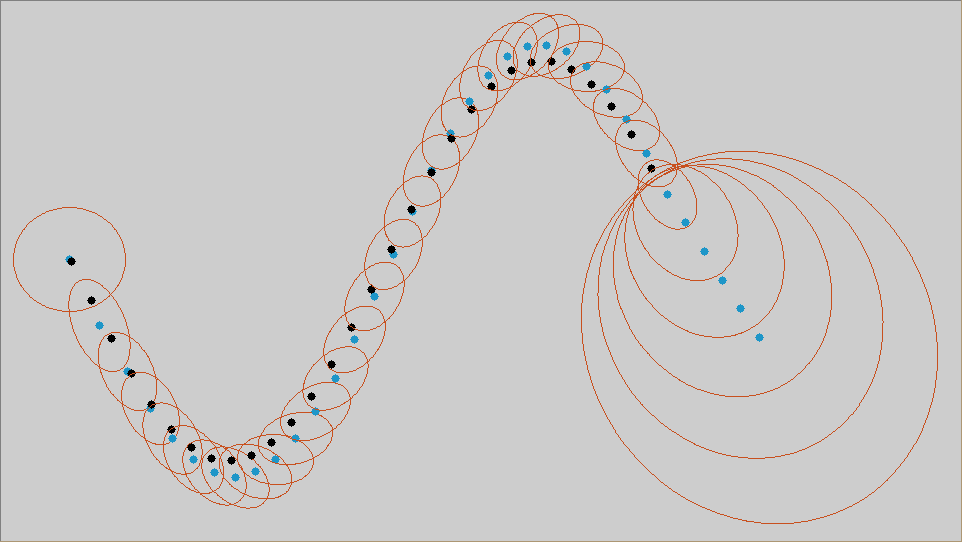
\includegraphics[width=\linewidth]{images/Kalmask2}
	\caption{\textit{Kalman Prediction figure.}}
	\label{fig:kalman_fig} %Skapar referens till figuren
\end{figure}